\begin{frame}{$k$-NN -- method summary}

% \maketag{Supervised} 
\maketag{regression} \maketag{classification}
\maketag{Nonparametric} \maketag[50]{White-box}

\medskip

\highlight{General idea}
\begin{itemize}
  \item Rationale: \textbf{similarity} in feature space $\leadsto$ similarity 
  in target space w.r.t. certain \textbf{metric}
  % \item The \textbf{$k$-nearest neighbors ($k$-NN)} model is based on 
  % inter-observational \textbf{distances}, thus heavily depending on the chosen 
  % \textbf{distance measure}.
  \item \textbf{Prediction} for $\xv$: construct \textbf{$k$-neighborhood} 
  $N_k(\xv)$ from $k$ points closest to $\xv$ in $\Xspace$, then 
  predict
  \begin{itemize}
    \footnotesize
    \item (weighted) mean target for \textbf{regression}: 
    $\left. \yh = 1 \middle/ 
    (\sum_{i: \xi \in N_k(\xv)} w_i) \sum_{i: \xi \in N_k(\xv)} w_i \yi \right.$
    \item most frequent class for \textbf{classification}: 
    $\yh = \argmax_{\ell \in \gset} \sum_{i: \xi \in N_k(\xv)} \I(\yi = \ell)$
  \end{itemize}
  \item No distributional or functional \textbf{assumptions}
  \item \textbf{Nonparametric} behavior: parameters = training data; no 
  compression of information
  \item Not immediately interpretable, but inspection of neighborhoods revealing
\end{itemize}

\medskip

\highlight{Hyperparameters} ~~ Neighborhood \textbf{size} $k$ (locality), 
\textbf{distance} measure

\vfill

\begin{minipage}{0.7\textwidth}
  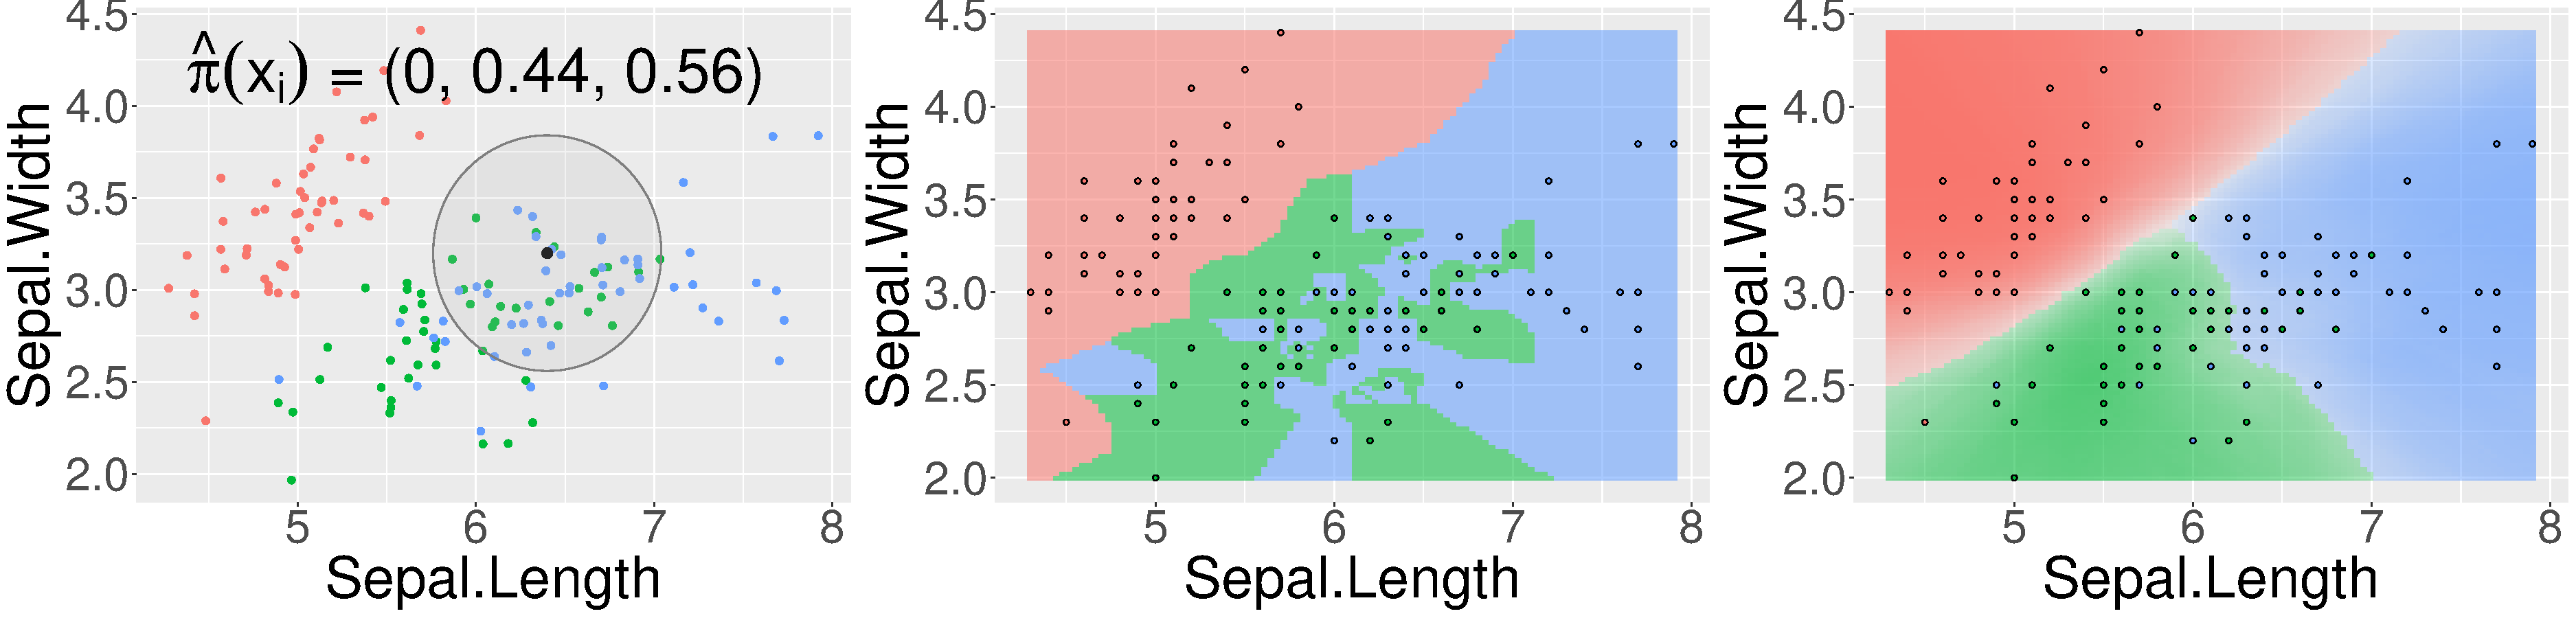
\includegraphics[width=\textwidth]{figure/knn-neighborhood.pdf}
\end{minipage}%
\hfill
\begin{minipage}{0.25\textwidth}
  \tiny
  \raggedright
  \textit{Left}: Neighborhood for exemplary observation in \texttt{iris}, 
  $k = 50$ \\
  \textit{Right}: Prediction surfaces for $k \in \{1, 50\}$
\end{minipage}
\end{frame}

% ------------------------------------------------------------------------------

\begin{frame}{$k$-NN -- Pro's \& Con's}

\footnotesize

\begin{columns}[onlytextwidth]
  \begin{column}{0.5\textwidth}
    \highlight{Advantages}
    \footnotesize
    \begin{itemize}
      \positem Algorithm \textbf{easy} to explain and implement
      % \positem Applicable to both regression and classification
      \positem No functional \textbf{assumptions} -- therefore (in theory) able 
      to model data situations of \textbf{arbitrary complexity}
      \positem No \textbf{training} period
      \positem No \textbf{optimization} required 
      \positem Constant evolvement with \textbf{new data}
      \positem Ability to learn \textbf{nonlinear} decision boundaries
      \positem Easy to \textbf{tune}
      % \positem Only one \textbf{hyperparameter} to tune
    \end{itemize}
  \end{column}
  \begin{column}{0.5\textwidth}
    \highlight{Disadvantages}
    \footnotesize
    \begin{itemize}
      \negitem Sensitivity w.r.t. \textbf{noisy} or \textbf{irrelevant} features
      and outliers due to utter reliance on distances
      \negitem Bad performance when feature \textbf{scales} not consistent 
      with importance
      \negitem Heavily afflicted by \textbf{curse of dimensionality}
      \negitem No handling of \textbf{missing} data
      \negitem Poor handling of data \textbf{imbalances} (worse for more global 
      model, i.e., large $k$)
      \negitem High \textbf{memory} consumption of distance computation
    \end{itemize}
  \end{column}
\end{columns}

\vfill

\small

\conclbox{Easy and intuitive for small, well-behaved datasets with meaningful 
feature space distances}

\end{frame}

% ------------------------------------------------------------------------------

\begin{frame}{$k$-NN -- Practical hints}

\highlight{Popular distance measures}

\begin{itemize}
  \item Numerical features: typically, \textbf{Minkowski} distances
  $d(\xv, \xtil) = \|\xv - \xtil \|_q = 
  \left( \sum_j | x_j - \tilde{x_j} |^q
  \right)^{\tfrac{1}{q}}$
  \begin{itemize}
    \item $q = 1$: \textbf{Manhattan} distance $\rightarrow d(\xv, \xtil) =
    \sum_j | x_j - \tilde{x_j} |$
  \item $q = 2$: \textbf{Euclidean} distance $\rightarrow d(\xv, \xtil) =
  \sqrt{\sum_j (x_j - \tilde{x_j})^2}$
  \end{itemize}
  \item In presence of categorical features: \textbf{Gower} distance
  \item \textbf{Custom} distance measures applicable
  \item Optional \textbf{weighting} to account for beliefs about varying feature
  importance
\end{itemize}

\medskip

\highlight{Implementation}
\begin{itemize}
  \item \textbf{R:} \texttt{mlr3} learners \texttt{LearnerClassifKKNN} /
  \texttt{LearnerRegrKKNN}, calling \texttt{kknn::kknn()}
  \item \textbf{Python:} \texttt{KNeighborsClassifier} / 
  \texttt{KNeighborsRegressor} from package \texttt{scikit-learn}
\end{itemize}

\end{frame}